% Source: https://tex.stackexchange.com/a/561260/6880

\documentclass[tikz, border=2mm]{standalone}

\usetikzlibrary{positioning}

\tikzset {
    node distance=.1cm,
    one/.style={
        draw,
        minimum size=1cm,
        inner sep=0pt
        },
    tenthv/.style={
        draw,
        minimum height=1cm,
        minimum width=0.1cm,
        inner sep=0pt,
    },
    tenthh/.style={
        draw,
        minimum height=0.1cm,
        minimum width=1cm,
        inner sep=0pt,
    },
    hundreth/.style={
        draw,
        minimum size=0.1cm,
        inner sep=0pt,
    },
   base graph/.pic={
        \node[one] (00) {};
        \node[one, below=of 00] (10) {};
        \node[tenthh, below=of 10] (20) {};
        \foreach \i [count=\xi, remember=\xi as \lasti (initially 0)] in {1,2,3,4} 
          \node[tenthv, right=of 0\lasti] (0\xi) {};         
        \path (00.north west) -- (20.south west) node[midway, left] {2.1} ;
        \path (00.north west) -- (04.north east) node[midway, above] {1.4} ;
        }
    }

\begin{document}

      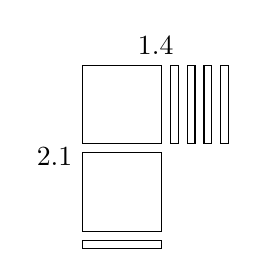
\begin{tikzpicture}
        \pic {base graph};
      \end{tikzpicture} 

      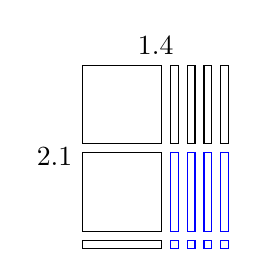
\begin{tikzpicture}
        \pic {base graph};
        \foreach \i [count=\xi] in {1,2,3,4} {
          \node[tenthv, blue, below= of 0\xi] (1\xi) {}; 
          \node[hundreth, blue, below= of 1\xi] (2\xi) {}; 
          }
      \end{tikzpicture}
\end{document}